\section{An Accurate Performance Model}
This section introduces a new performance model constructed to accurately predict the execution time of the MapReduce job in the Hadoop cluster.

To construct an accurate performance model, there are some effective methods and principles as follows:
\begin{itemize}
\item The execution procedure of the MapReduce job is complicated, which is determined by the configuration parameters, input data and so on. Therefore, an accurate performance predictor needs to forecast the MapReduce job's actual execution procedures.
\item The MapReduce job's execution consists of multiple phases , this performance model should be able to forecast accurately each phase's cost of the job.
\item It is essential to confirm whether the parallel exists between multiple phases, and to predict the overlap time between these phases executed in parallel.
\end{itemize}

The performance predictor consists of the following two sections.

\subsection{The Cost Model For Map Task}
The execution of the map task consists of the following phases: read, map, spill and merge. The key of our work is to predict the actual cost of map and spill.

\noindent\textbf{Map and Spill. }The user-defined map function is executed by the main thread to process the input data, and the spill of the buffer data is performed by the spill thread to sort, combine and write the buffer data sequentially.

\noindent\textbf{(i) Execution Procedure}
\begin{figure}[htbp]
\centering
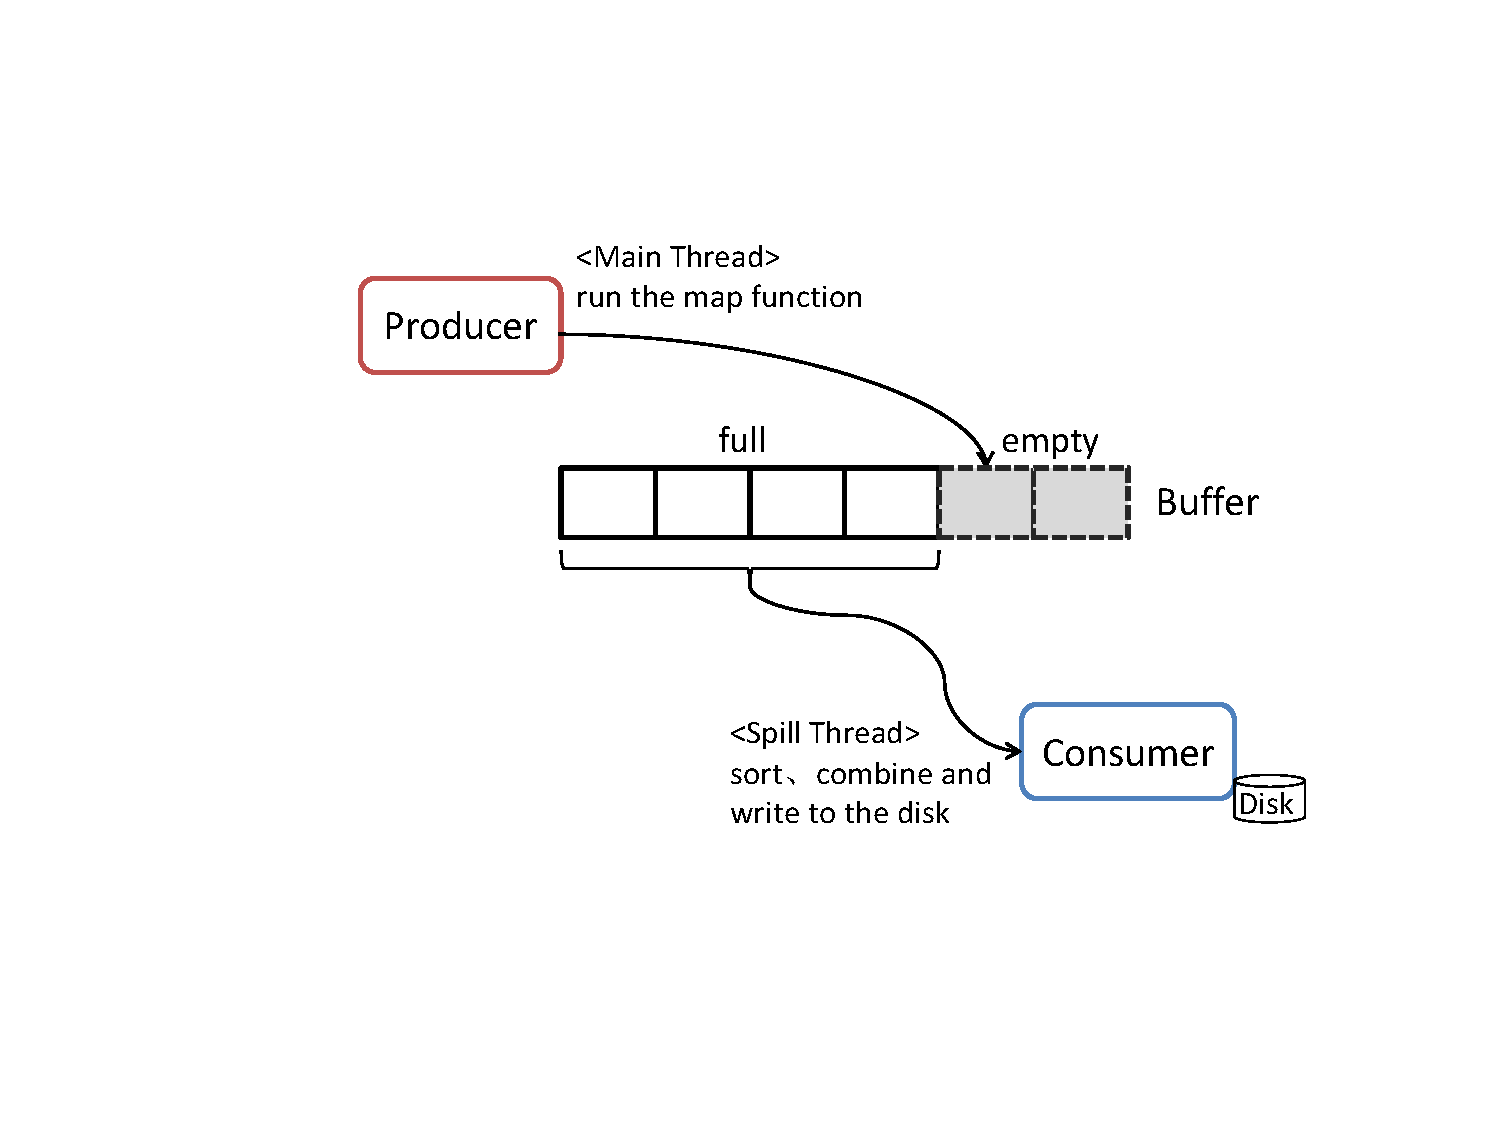
\includegraphics[height=4.5cm, width=8cm]{mapandspill}
\caption{The Interaction between Map and Spill}
\label{fig:inter}
\end{figure}

As shown in Figure \ref{fig:inter}, when the main thread executes the map function, the output of the map function is written into the memory buffer. The spill thread starts to spill the outputs cached in the buffer to the disk file, when the used space of the buffer reaches the threshold determined by the related configuration parameters. Meanwhile, the main thread continues to execute the map function util the buffer is full. 

\noindent\textbf{(ii) The Analysis of Key Effect Factors}
\begin{itemize}
\item  \textbf{The cost of map function's single execution} $csMapCost$, and \textbf{the number of map function's execution} $dMapInputRecs$. The factor $csMapCost$ is determined by not only the complexity of the user-defined map function but also the execution environment, such as the number of executing threads and the resource consumed by the map task.
\item  \textbf{The size of memory buffer} $pSortMB$, and \textbf{the threshold at which the spill is triggered} $pSpillPerc$. These two factors determine when to spill.
\end{itemize}

To predict the total cost of these two phases, we need to estimate not only the individual cost of map and spill, but also their overlap time during which these two phases execute simultaneously. The cost of map is determined by the $csMapCost$ and $dMapInputRecs$, and the cost of spill is determined by the cost of a single spill $cSpillCost$ and the number of spill affected by the $pSortMB$ and $pSpillPerc$. If the $pSortMB$ and $pSpillPerc$ increase, the $cSpillCost$ increases but the number of spill decreases, therefore it's uncertain whether the cost of spill increases or not. Their overlap time is determined by the $cSpillCost$ and the cost of map when spilling $cMapWithSpill$ which is also affected by the $pSortMB$ and $pSpillPerc$. When the $pSortMB$ is fixed, if the $pSpillPerc$ increases, the $cSpillCost$ increases but the $cMapWithSpill$ might decreases or increases(it's determined by whether the main thread is sleep or not), therefore it's also uncertain whether the overlap time increases or not. In summary, it's challenging to estimate the total execution time of map and spill which is nonlinearly affected by these key factors. We construct the following model to predict the total execution time of map and spill.


\noindent\textbf{(iii) The Construction of Model}

The spill thread spills the data cached in the buffer in parallel with the main thread which executes the map function. However, during the spill, the main thread starts to sleep when the buffer is full, and the main threads restarts to execute the map function when current spill is completed.

We separately estimate the actual execution cost of the map and spill as follows.

\noindent\textbf{1. The main thread sleeps}

When there are not enough remaining space in the buffer to hold the output of the map function during the spill, the main thread sleeps.
\begin{figure}[htbp]
\centering
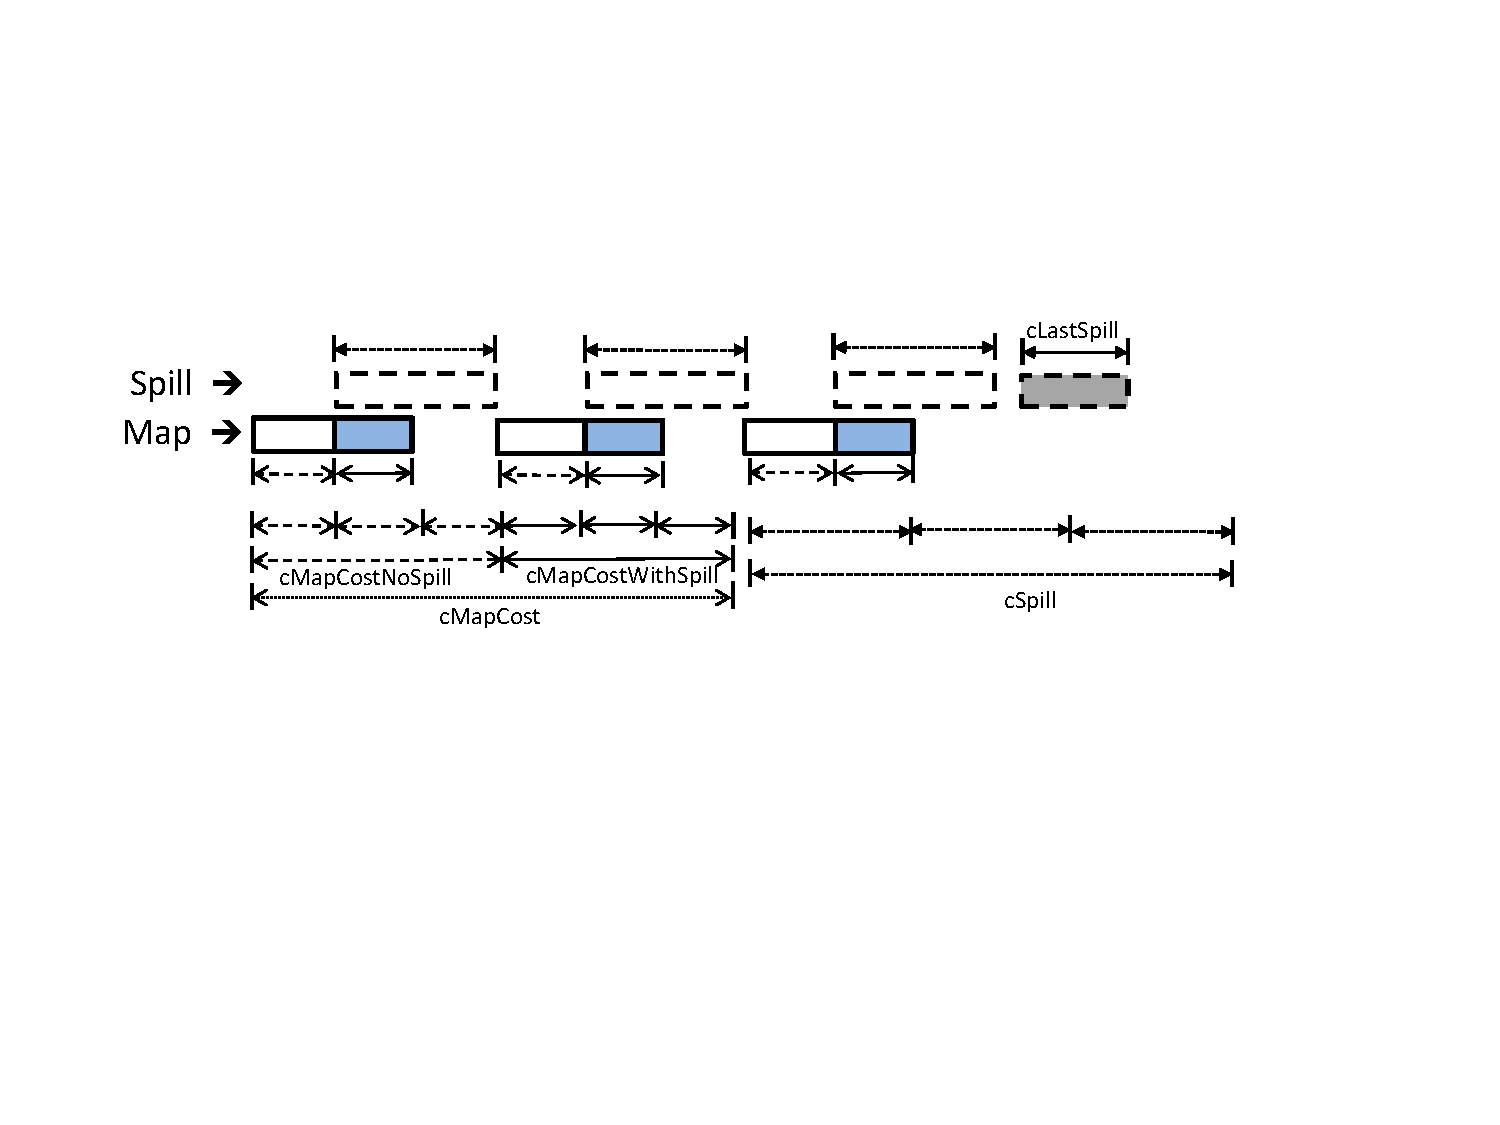
\includegraphics[height=3.5cm, width=8.5cm]{model1}
\caption{The Actual Cost of the Map and Spill(the main thread doesn't sleep)}
\label{fig:act}
\end{figure}

To predict the total execution time of these two phases $cMapAndSpill$, we have to estimate the costs of these two phases and their overlap time as follows.
\begin{small}
\begin{equation}
\begin{split}
cMapA&ndSpill=cSpillCost+cLastSpillCost \\
&+cMapCost-cOverTimeMapSpill
\end{split}
\end{equation}
\end{small}
where the $cSpillCost$ is the cost of all the spills except the last, the $cLastSpillCost$ is the cost of last spill executed by the main thread, the $cMapCost$ is the cost of the map, and the $cOverTimeMapSpill$ is the overlap time between these two phases.

\noindent\textbf{1.1 The cost of all the spills except the last: $cSpillCost$}

The $cSpillCost$ is estimated as follows.
\begin{small}
\begin{equation}
\begin{split}
cSpillCost=dNumSpills\times cOneSpillCost
\end{split}
\end{equation}
\end{small}
where the $dNumSpills$ is the number of spills executed by the spill thread, and the execution cost per spill $cOneSpillCost$ which is estimated as follows.
\begin{small}
\begin{equation}	
\begin{split}
cOneSpillCost=&dRecsPerSpill\times \frac{\sum_{i=1}^ncsSortCost_i}{n}\\
&+dRecsPerSpill\times \frac{\sum_{i=1}^ncsComCost_i}{n}\\
&+dSpillOutBytes\times \frac{\sum_{i=1}^ncsWriCost_i}{n} \nonumber
\end{split}
\end{equation}
\end{small}
where the $dRecsPerSpill$, $dRecsPerSpill$ and $dSpillOutBytes$ are estimated by the means introduced above, and the $csSortCost_i$, $csComCost_i$ and the $csWriCost_i$ are respectively the cost statistics about sorting, combining and writing.

\noindent\textbf{1.2 The cost of last spill: $cLastSpillCost$}

The cost of last spill $cLastSpillCost$ is estimated as follows.
\begin{small}
\begin{equation}
\begin{split}
cL&astSpillCost=(dMapOutRecs-dNumSpills\\
&\times  dRecsPerSpill)\times \frac{\sum_{i=1}^ncsSortCost_i}{n}+(  \\
&dMapOutRecs-dNumSpills\times dRecsPerSpill\\
&)\times \frac{\sum_{i=1}^ncsComCost_i}{n}+dMapOutRecWidth\times  \\
&(dMapOutRecs-dNumSpills\times dRecsPerSpill\\
&)\times \frac{\sum_{i=1}^ndsComSizeSel_i}{n}\times \frac{\sum_{i=1}^ncsWriCost_i}{n}
\end{split}
\end{equation}
\end{small}
where the $cLastSpillCost$ is composed of the costs of sorting, combining and writing the buffer data into a new disk file, and the $csComCost_i$ is the data statistics about combining. 

\noindent\textbf{1.3 The cost of map: $cMapCost$}

Through the above analysis of the key effect factors, the cost of map function's execution every time is effected by the number of executing threads in the map task. The main thread may execute the map function when the spill thread is spilling the data cached in the buffer into a new file, and the execution speed of the map function is slower due to the simultaneous execution of the spill thread. Therefore, the execution cost of map is divided into two parts as follows.
\begin{small}
\begin{equation}
\begin{split}
cMapCost=cMapCostWithSpill+cMapCostNoSpill
\end{split}
\end{equation}
\end{small}
where the $cMapCost$ is the total execution time of map, the $cMapCostWithSpill$ is the execution time of map when the spill thread is running and the $cMapCostNoSpill$ is the execution time of map when the spill thread is stopping. And the $cMapCostWithSpill$ and $cMapCostNoSpill$ are estimated as follows.
\begin{small}
\begin{equation}
\begin{split}
c&MapCostWithSpill=cMapCostWithOneSpill\times \\
&(dNumSpills-1)+Min(\frac{pSortMB\times (1-pSpillPerc)}{(dMapOutRecWidth+16)} \\
&,dMapOutRecs-dRecsPerSpill\times dNumSpills)\times \\
&\frac{\sum_{i=1}^ncsMapCostWithSpill_i}{\sum_{i=1}^ndsMapRecsSel_i} \nonumber
\end{split} 
\end{equation}
\end{small}
\begin{small}
\begin{equation}
\begin{split}
&cMapCostNoSpill=(dMapOutRecs-(dNumSpills-1 \\
&)\times\frac{pSortMB\times (1-pSpillPerc)}{(dMapOutRecWidth+16)}-Min(dMapOutRecs - \\
&dRecsPerSpill\times dNumSpills, \frac{pSortMB}{(dMapOutRecWidth+16)} \\
&\times (1-pSpillPerc)))\times \frac{\sum_{i=1}^ncsMapCost_i}{\sum_{i=1}^ndsMapRecsSel_i} \nonumber
\end{split}
\end{equation}
\end{small}
where the $csMapCost_i$ is the cost of map function's execution every time when the spill thread is not running on the $i$th machine, and it is captured by the LTrace. The  $cMapCostWithOneSpill$ is the cost of the map when the spill thread is executing, and it is estimated as follows.
\begin{small}
\begin{equation}
\begin{split}
cMapCostWithOneSpill&=\frac{pSortMB\times (1-pSpillPerc)}{(dMapOutRecWidth+16)} \\
&\times\frac{\sum_{i=1}^ncsMapCostWithSpill_i}{\sum_{i=1}^ndsMapRecsSel_i} \nonumber
\end{split}
\end{equation}
\end{small}
\emph{where the $csMapCostWithSpill_i$ is the cost of map function's execution every time when the spill thread is running on the $i$th machine, and it is captured by the LTrace.}

\noindent\textbf{1.4 The overlap time: $cOverTimeMapSpill$}

At last, the $cOverTimeMapSpill$ is estimated as follows.
\begin{small}
\begin{equation}
\begin{split}
cOverTimeMapSpill=cMapCostWithSpill
\end{split}
\end{equation}
\end{small}
As show in the Figure \ref{fig:act}, the overlap time of the map and spill is just the $cMapCostWithSpill$, which has been estimated above.

\noindent\textbf{2. The main thread doesn't sleep} 

When there are enough remaining space in the buffer to hold the output of the map function during the spill, the main thread doesn't sleep.
\begin{figure}[htbp]
\centering
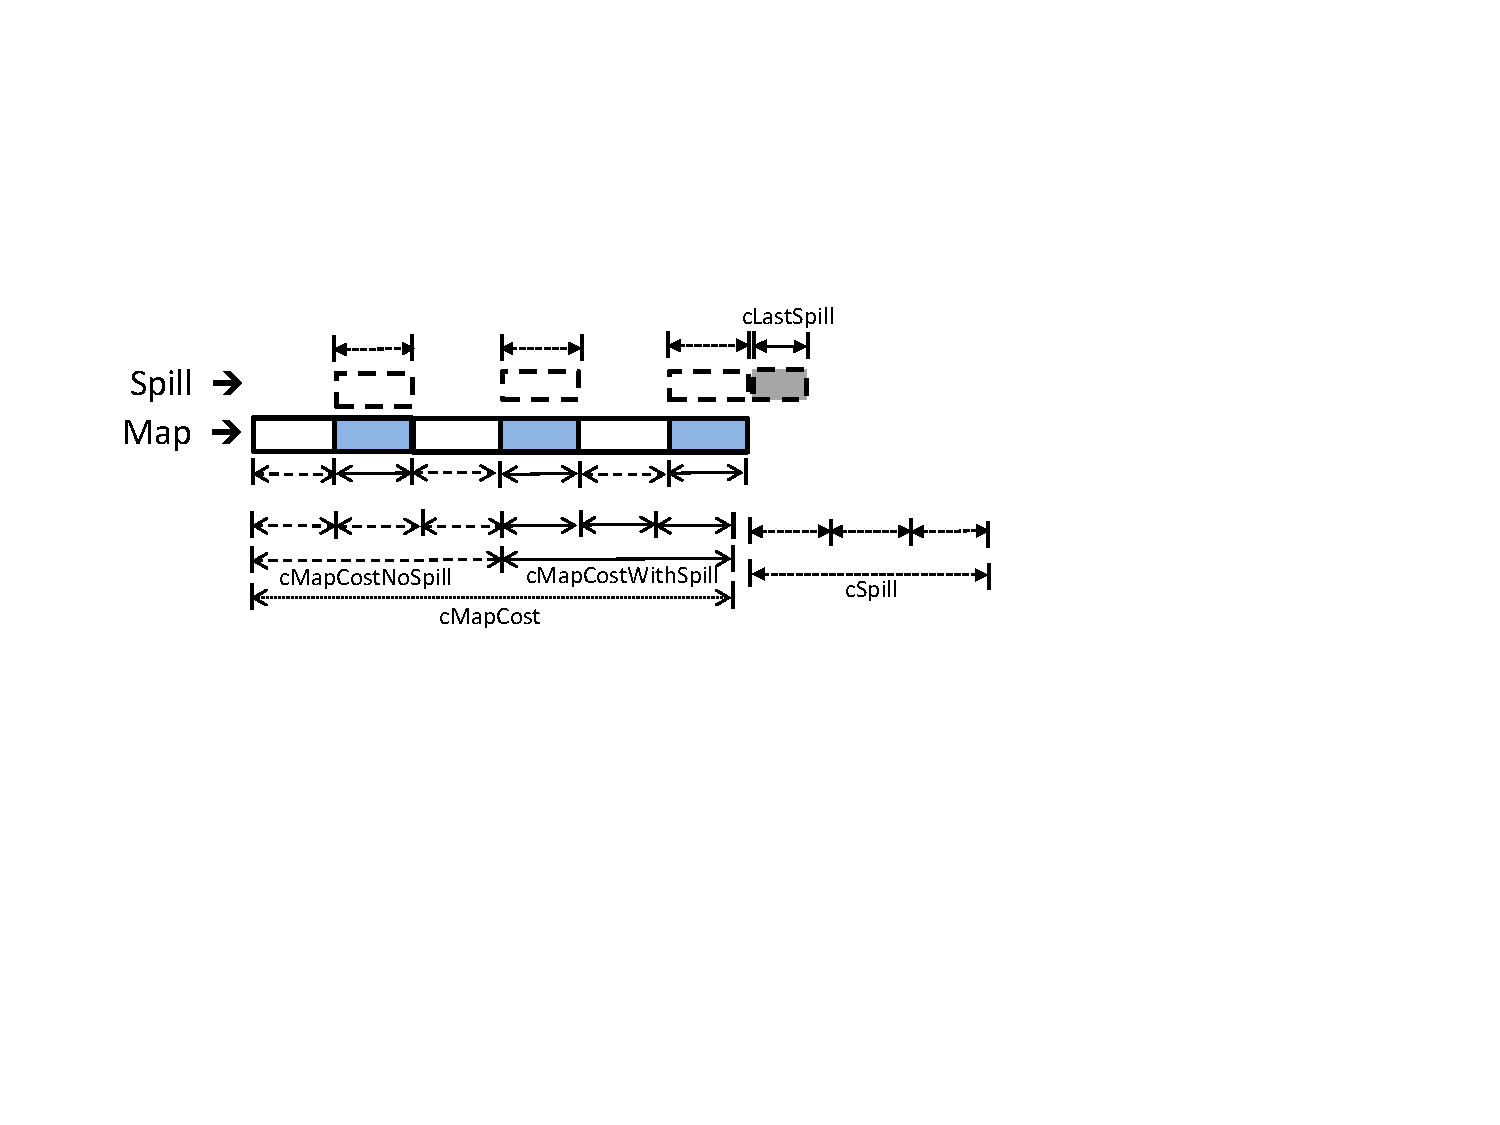
\includegraphics[height=3.5cm, width=9cm]{model2}
\caption{The Actual Cost of the Map and Spill(the main thread  sleeps)}
\label{sleeps}
\end{figure}

We can estimate the $cSpillCost$, $cLastSpillCost$, $cOverTimeMapSpill$ as described previously. However, when the main thread doesn't sleep, we need estimated the $cMapCostWithSpill$ and $cMapCostNoSpill$ as follows.
\begin{small}
\begin{equation}
\begin{split}
cMapCostWithSpill=dN&umMapsWithSpill \\
&\times\frac{\sum_{i=1}^ncsMapCostWithSpill_i}{n} \nonumber
\end{split}
\end{equation}
\end{small}
\begin{small}	
\begin{equation}
\begin{split}
cMapCostNoSpill=dNumMapsNoSpill\times \frac{\sum_{i=1}^n csMapCost_i}{n} \nonumber
\end{split}
\end{equation}
\end{small}
where the $dNumMapsWithSpill$ is the number of map function's execution when the spill thread is running, and the $dNumMapsNoSpill$ is the number of map function's execution when the spill thread is sleeping, and they are estimated as follows.
\begin{small}
\begin{equation}
\begin{split}
d&NumMapsWithSpill=\frac{cOneSpillCost\times n}{\sum_{i=1}^n csMapCostWithSpill_i} \times \\
&(dNumSpills-1)+Min( \frac{cOneSpillCost\times n}{\sum_{i=1}^n csMapCostWithSpill_i} \\
&, \frac{(dMapOutRecs-dNumSpills\times dRecsPerSpill)\times n}{\sum_{i=1}^ndsMapRecsSel_i})  \nonumber
\end{split}
\end{equation}
\end{small}
\begin{small}
\begin{equation}
\begin{split}
dNumMapsNoSpill=dMapI&nputRecs-	\\
				&dNumMapsWithSpill \nonumber
\end{split}
\end{equation}
\end{small}
The $dMapInputRecs$ is just the total number of map function's execution.



\subsection{The Cost Model For Reduce Task}
The execution of the reduce task, which is described in the section 2, consists of the following phases: shuffle, merge, reduce and write. The key of our work is to predict the effective cost of shuffle.

\noindent\textbf{Shuffle.} The reduce task reads the corresponding outputs of all the map tasks from the remote machines in the cluster.

\noindent\textbf{(i) Execution Procedure}
\begin{figure}[htbp]
\centering
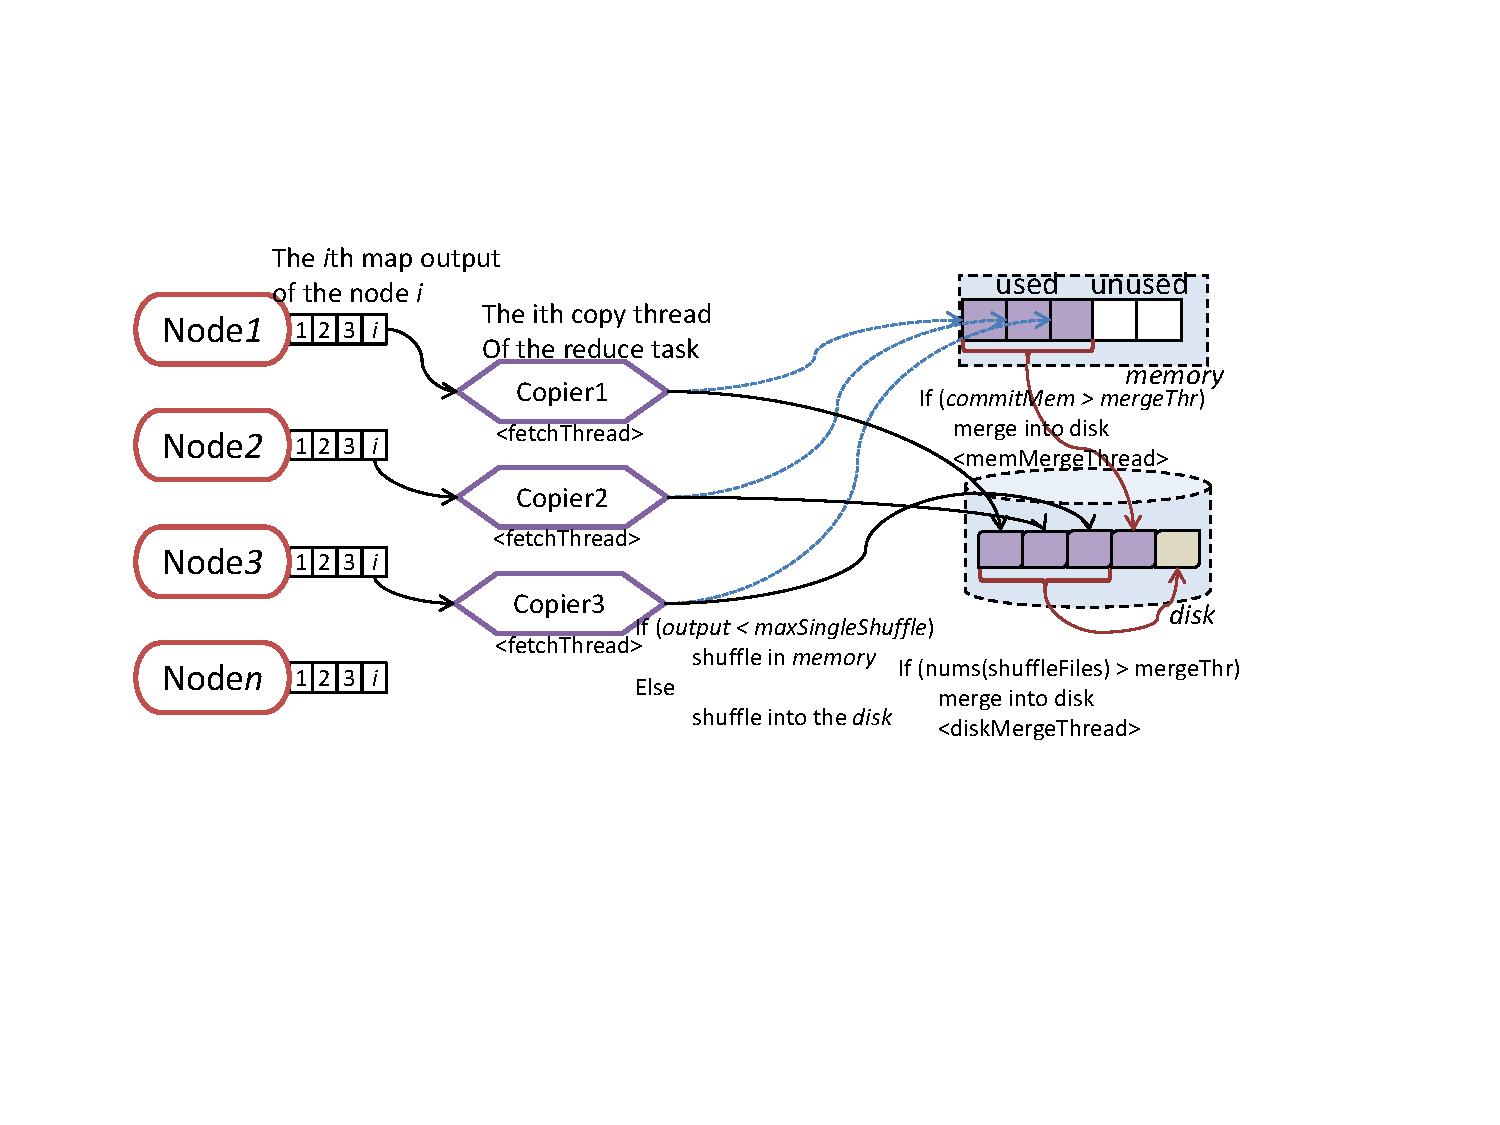
\includegraphics[height=4.5cm, width=9cm]{shuffle}
\caption{The Execution Procedure of Shuffle}
\label{fig:proce}
\end{figure}

As shown in Figure \ref{fig:proce}, multiple copy threads of the reduce task are started to simultaneously fetch the corresponding outputs of map tasks from the various machines. When there are multiple outputs generated by different map tasks on a machine, only one of these copy threads sequentially fetches these outputs from the target machine.

When the copy thread starts to fetch the output of the completed map task, the output may be written to the memory buffer or a new disk file, which is determined by the way as shown in figure 4. A merge thread is started, when the used space of the memory buffer or the number of disk files reach the threshold.

\noindent\textbf{(ii) The Analysis of Key Effect Factors}
\begin{itemize}
\item \textbf{The number of copy threads} $numCopies$, the $numCopies$ is the actual number of copy threads , and these threads simultaneously fetch the outputs of map tasks from $numCopies$ machines.
\item \textbf{The output of the map task} $mapOutputs$, and \textbf{the max single shuffle limit} $maxSinShufLimit$. These two factors determine whether the map task's output is fetched into the buffer or disk.
\item \textbf{The threshold at which the memory merge is triggered} $mergeThreshold$, and \textbf{the number of disk files at which the disk merge is triggered} $pSortFactor$. These two factors affect when the merge thread merge the buffer data or the disk files into a new file, when the 
\end{itemize}

\noindent\textbf{(iii) The Estimation of the Execution Cost}

The shuffle of the reduce task may be completed together by multiple threads, such as multiple copy threads, the memory merge thread and the disk merge thread. When the reduce task starts, multiple copy threads are started to fetch the map tasks' outputs. A memory merge thread is started to merge the outputs within the buffer to a new file, when the size of used buffer reaches the merge threshold. And a disk merge thread is started to merge the disk files into a new file, when the number of disk file reaches the disk merge threshold.	

\begin{figure}[htbp]
\centering
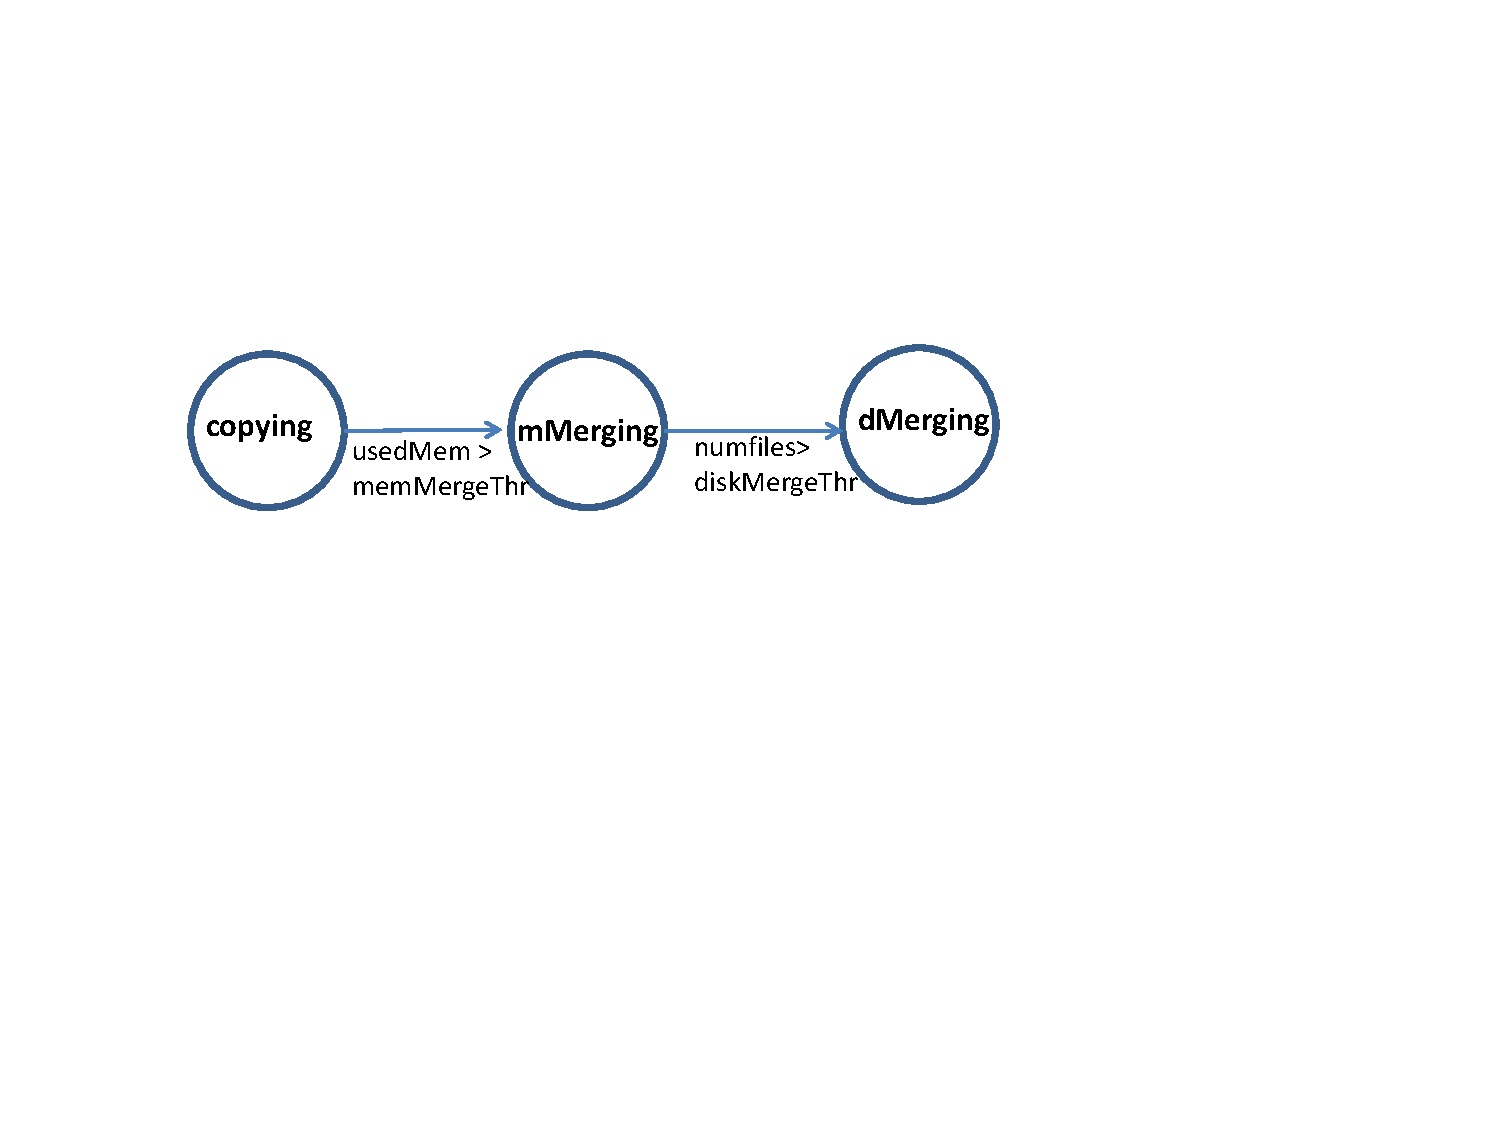
\includegraphics[height=1.75cm, width=7.7cm]{status}
\caption{The State Transition Graph of the Shuffle}
\label{fig:state}
\end{figure}

In the phase of spill, the state transition of the above three threads is shown as the Figure \ref{fig:state}.  The copy thread starts to copy, when the reduce task starts. And the copy thread stops, when the copy is completed. The memory merge thread is triggered to execute the memory merge, when the used memory is greater than memory merge threshold, and used memory is determined by the copy thread. The disk merge thread is triggered to execute the disk merge, when the number of disk files is greater than the disk merge threshold, and the number of disk files is determined by the memory thread. The start time of the shuffle is the start time of copy thread, and the end time of the shuffle is the maximum end time of the copy thread, memory merge thread and disk merge thread.


We propose the simulation approach to predict the whole shuffle time of the reduce task. 

\noindent\rule{3.5in}{0.6mm}
\textbf{Algorithm 1} The simulation of shuffling into the buffer
\rule{3.5in}{0.3mm}
\begin{algorithmic}[1]
\Require $mapOutputs$, $numCopies$
\Ensure $cShuffleTime$
\Function{CShMCost}{$mapOutputs, numCopies$}
\State // $T_c$, $T_m$, $T_d$ are the clock of copy, memory merge and disk merge threads
\State $T_c \gets 0, T_m \gets 0, T_d \gets 0$
\While{!\Call{IsNull}{$mapOutputs$}}


\State //the $numCopies$ threads copy $mapOutputs$
\For{$t=0 \to numCopies - 1$}
\If{$t < length(mapOutputs) $}
\State $Outs_m \gets Outs_m + mapOutputs[t]$
\State //maintain the $mapOutputs$ 
\EndIf
\EndFor

\State $T_c \gets T_c + \Call{ShuCost}{mapOutputs[0]}$
\If{\Call{IsMerge}{$Outs_m$}}
\State // memory merge
\State $T_m \gets \Call{Max}{T_c, T_m}$
\State $T_m \gets T_m + \Call{MemMerge}{Outs_m, numOuts_{mtod},Outs_d}$

\If{$\Call{IsDiskMerge}{Outs_d}$}
\State // disk merge
\State $T_d \gets \Call{Max}{T_d, T_m}$
\State $T_d \gets \Call{DiskMerge}{Outs_d} + T_d$
\EndIf
\EndIf

\If{\Call{IsFull}{$Outs_m$}}
\State $\Call{RemoveMemOuts}{Outs_m, $
$numOuts_{mtod}}$
\State $T_c = \Call{Max}{T_c, T_m}$
\EndIf

\EndWhile
\State $cShuffleTime \gets \Call{Max}{T_c, T_m, T_d}$
\EndFunction
\end{algorithmic}
\noindent\rule{3.5in}{0.6mm}

In the algorithm 1, the $mapOutputs$ and $numCopies$ are the input of the algorithm. The $mapOutputs$ is the outputs of map tasks on all the machines,  each element of $mapOutputs$ records the number of map tasks on the one machine and the size of each map task's output. The $numCopies$ is the number of copy threads within a map task. The $cShuffleTime$ is the output, and it represents the cost of the shuffle within the reduce task. At line 3, the $T_c$, $T_m$ and $T_d$ respectively are the clock of copy thread, memory merge thread and the disk merge thread, and these clocks record the start or end time of the related trigger event. For example, the $T_m$ records the start and end time of the memory merge executed by the memory merge thread. From line 5 to line 12,  the $numCopies$ copy threads respectively fetch one map task's output to the memory buffer from $numCopies$ machines, the $Outs_m$ is the outputs of map tasks within the memory buffer, and the $T_c$ will increase by the cost of one copy.  Line 13 to 16, the memory merge thread merge the memory buffer data into a disk file, if the size of buffer data reaches the merge threshold. And the $T_m$ will increase by the cost of one memory merge. Line 17 to 21, the disk merge thread merge merge the disk files into a new disk file, if the number of the disk files reaches the merge threshold. And the $T_d$ will increase by the cost of one disk merge. At Line 28, The $cShuffleTime$, the cost of shuffle, is the maximum of $T_c$, $T_m$, $T_d$.

Similar to the algorithm 1, we can use the similar method to calculate the cost of the shuffle, when the map tasks' outputs are written into the disk.  The $T_c$ and $T_d$ respectively are the clock of copy thread and disk merge thread, and the maximum of the $T_c$ and $T_d$ is the shuffle cost $cShuffleTime$.

